\begin{figure}[H]
\begin{center}
	The best move for Left is selecting the purple cheque equal to \gam{1}{{-}1}
	\vspace{0.5cm}
	
	\begin{tikzpicture}
		\begin{scope} []
			\draw[fill=yellow] (-1,-1) rectangle ++(6,1.9);
			\node[circle, draw, fill=purple2] at (0,0) {1 $|$ 1};
			\node[circle, draw, fill=purple2] at (2,0) {4 $|$ 2};
			\draw[thick] (3,-0.75) -- (3,0.75);
			\node[circle, draw, fill=purple2] at (4,0) {{-}9 $|$ 9};
			\node[draw,fill=blue, circle] at (1,-2) {};
			\node[draw,fill=blue, circle] at (0.5,-1.5) {};
		\end{scope}
	\end{tikzpicture}
\end{center}
\end{figure}
\begin{figure}[H]
\begin{center}
	The best move for Left is selecting the purple cheque equal to \gam{4}{{-}2}
	\vspace{0.5cm}
	
	\begin{tikzpicture}
		\begin{scope} []
			\draw[fill=yellow] (-1,-1) rectangle ++(6,1.9);
			\node[circle, draw, fill=purple2] at (0,0) {1 $|$ 1};
			\node[circle, draw, fill=purple2] at (2,0) {4 $|$ 2};
			\draw[thick] (3,-0.75) -- (3,0.75);
			\node[circle, draw, fill=purple2] at (4,0) {{-}9 $|$ 9};
			\node[circle, draw, fill=purple2] at (2,-2) {4 $|$ 4};
		\end{scope}
	\end{tikzpicture}
\end{center}
\end{figure}
\begin{figure}[H]
	\begin{center}
		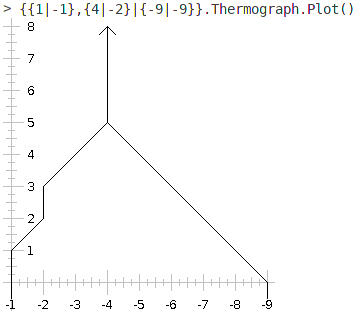
\includegraphics[scale=0.5]{sections/temperature/g1Therm.png}
		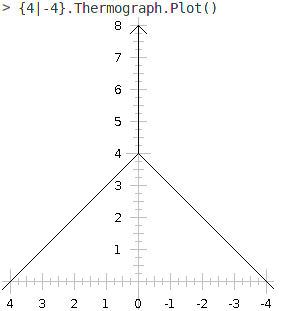
\includegraphics[scale=0.5]{sections/temperature/g2Therm.png}
	\end{center}
\caption{Complete example of the best move changing}
\end{figure}